\section{Implementation}

\subsection{Overview}
Our system has been implemented using GAE (Google App Engine) and Android to construct an App Engine Connected Android Application.  
The justification for using Android is detailed in Section \ref{sec:Mobile}.
GAE was used for the backend of our system for two reasons, firstly because members of the team had prior experience in using this system. 
Secondly because support for this project is provided by Eclipse; which generates a starter project with the following implementations \cite{AppEngine}:
\begin{itemize}
	\item{Handling communication between the service and application}
	\item{Registering and unregistering with the service}
	\item{Authentication and user accounts}
	\item{Transferring of data between the application and datastore to allow use of the same classes}.
\end{itemize}

\subsection{Architecture}
The overall architecture of such an application is given by the diagram below:

\begin{figure}[ht]
\begin{center}
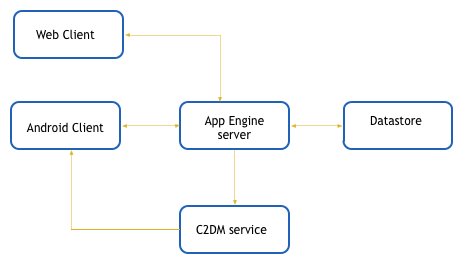
\includegraphics[trim = 0mm 0mm 0mm 0mm, clip, scale=0.7]{images/arch.png}
\caption{Architecture Diagram \cite{AppEngine}} 
\end{center}
\end{figure}

From this architecture the following modules have been implemented: 
\begin{itemize}
	\item{The \textbf{Android} application.}
	\item{The \textbf{GAE} including the \textbf{Datastore}.}
	\item{A basic implementation of the \textbf{Web Client} \cite{implementation} (which could be expanded as part of the future work, see Section \ref{sec:Web}.}
\end{itemize}

The C2DM (Cloud to Device Messaging) service which facilitates sending messages to Android devices from the cloud system is an additional service provided by Google \cite{implementation}. 

\subsection{Google App Engine}
The GAE backend was implemented in Java and is split into a number of components: the Datastore and Remote Procedure Call (RPC) service

\subsubsection{Datastore}
The first component is the database, which is implemented using GAE’s implementation of Java Data Objects (JDO). 
The objects that have been created to store information in the system are detailed in the following table:

\begin{table}[ht]
\begin{tabular}{|p{110pt}|p{200pt}|p{110pt}|}
\hline
Name			& Purpose		 									& Example	
\\\hline
CaffeineSource		& To model a location where caffeine products are sold.	& Avenue Cafe.
\\\hline
CaffeineProduct	& To model a unique caffeine product containing information such as name, type and milligrams of caffeine in product.	& Red Bull Can
\\\hline
CaffeineSourceProduct	& To model a unique caffeine product being sold at a location extending the referenced CaffeineProduct to include pricing information at this location.	& Red Bull Can at \newline Avenue Cafe.
\\\hline
OpeningTime		& To model a opening time for a location.	& Monday’s opening hours are between 8:00 and 19:00 for the period 00:00:00 16/4/12 to 23:59:59 15/6/12. 
\\\hline
LeaderboardScore	& To model a user’s score for leaderboard purposes.	&
\\\hline
\end{tabular}
\caption{Table detailing System Objects}
\end{table}

Additionally other objects may exist in the database such as DeviceInfo and C2DMConfig which are automatically added by the system to allow Cloud to Device Messaging (C2DM) which hasn't been created by the team. 

All of the location information used in Opticaff is retrieved using SPARQL queries on the University of Southampton’s SPARQL endpoint \cite{SotonSparql}. The datastore is evaluated daily to ascertain if it needs re-populating. This is done through the use of a scheduled task (cron job) and HTTPServlet which checks if the information currently stored is valid (e.g location opening times haven't expired) and if so performs the necessary dropping and adding of information to ensure the data is kept up-to-date.

Create, Read, Update and Delete (CRUD) operations have also been created to handle the tasks involved in the cron job service as well as the RPC service which is detailed in the next section.

The University of Southampton's data is stored is so that the application doesn't have to perform SPARQL queries on the fly and process them on every user request (e.g nearest caffeine source locations). Additionally the use of a JDO datastore is because it allows both the Android application and datastore to use the same Java objects and provides the means to transfer and use data easily.

\subsubsection{RPC Service}
The RPC service acts as an interface to the datastore for the Android Application and Web Client; communicating with this service is done using Google Accounts which handles the authentication process and user accounts meaning that to use our system it's necessary to have a Google account furthermore it means we don't have to store user account information in our datastore. 

This service contains a number of RPC methods which perform query actions on the datastore to provide Datastore objects information such as top 5 players on our leaderboards and nearest caffeine source locations and information for those sources.

\subsection{Support and Libraries Used}
Libraries and sources of information which were used to construct this project are listed below:
Google App Engine Documentation
Android Documentation
Jena Library 
To perform SPARQL queries and process results in GAE.
(http://incubator.apache.org/jena/index.html)
How to read calendar on phone in Android.
http://stackoverflow.com/questions/7859005/how-to-read-and-edit-android-calendar-events-using-the-new-android-4-0-ice-cream
How to create alarm events in Android.
http://justcallmebrian.com/?p=129
How to create Progress Dialog in Android.
http://www.helloandroid.com/tutorials/using-threads-and-progressdialog

\subsection{Implementation Problems}
During development a few problems were encountered:
\begin{itemize}
	\item{When running the Local App Engine server, an issue occurs when using a new version of java due to the removal of a getDefaultTimezone method. A solution was given in \cite{solution} and this was followed successfully.}
	\item{When testing the GAE Connected Android Project; the application was unable to obtain the debug url for the Local GAE. A solution was found here \cite{solution2} and followed.}
\end{itemize}
